\index{Rozenkruisers}\index{Substitutie!Symbolen}Een andere vorm van substitutie is het vervangen van letters en cijfers door symbolen. E\'en van de bekende vormen is die van de Rozenkruisers. de oudste variant is afkomstig uit 1533 en is beschreven in de \textquote{occulta philosophia} van Agrippa\index{Agrippa} von Nettesheim. Agrippa was een geleerd man uit Duitsland, geboren in Keulen in 1486 en gestorven in Grenoble in 1535. Zijn code kan beschreven worden zoals weergegeven in figuur \ref{fig:rosenkruisen}.

\begin{figure}[h!]
	\centering
	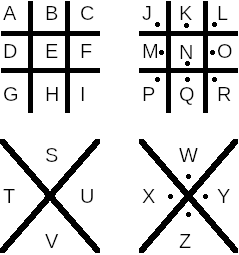
\includegraphics[width=0.4\linewidth]{Rozenkruisen.png}
	\caption{Rosenkruiserscode}
	\label{fig:rosenkruisen}
\end{figure}

Het deel waar de letter in staat is het symbool waardoor de letter vervangen wordt. Een a wordt dus een 

\includegraphics[height=\fontcharht\font`\B]{Rozenkruisen_A.png}
en een W wordt dan 

\includegraphics[height=\fontcharht\font`\B]{Rozenkruisen_W.png}
. Zo kunnen we ook zinnen maken, probeer maar eens uit te vinden wat hier staat:


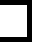
\includegraphics[height=\fontcharht\font`\B]{Rozenkruisen_d.png} 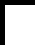
\includegraphics[height=\fontcharht\font`\B]{Rozenkruisen_i.png} 
\includegraphics[height=\fontcharht\font`\B]{Rozenkruisen_t.png} \, 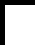
\includegraphics[height=\fontcharht\font`\B]{Rozenkruisen_i.png} 
\includegraphics[height=\fontcharht\font`\B]{Rozenkruisen_s.png} \, 
\includegraphics[height=\fontcharht\font`\B]{Rozenkruisen_e.png} 
\includegraphics[height=\fontcharht\font`\B]{Rozenkruisen_e.png} 
\includegraphics[height=\fontcharht\font`\B]{Rozenkruisen_n.png} \, 
\includegraphics[height=\fontcharht\font`\B]{Rozenkruisen_z.png} 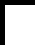
\includegraphics[height=\fontcharht\font`\B]{Rozenkruisen_i.png} 
\includegraphics[height=\fontcharht\font`\B]{Rozenkruisen_n.png}.

Hoewel minder makkelijk leesbaar is de decodering ook hier weer simpel omdat voor elke letter het symbool uniek is, dus er zijn maar 26 verschillende symbolen. Met voldoende tekst is deze versleuteling eenvoudig te kraken.

